\begin{appendices}

\chapter{HLF dataset features distribution}
\begin{figure}[hpt!]
  \centering
  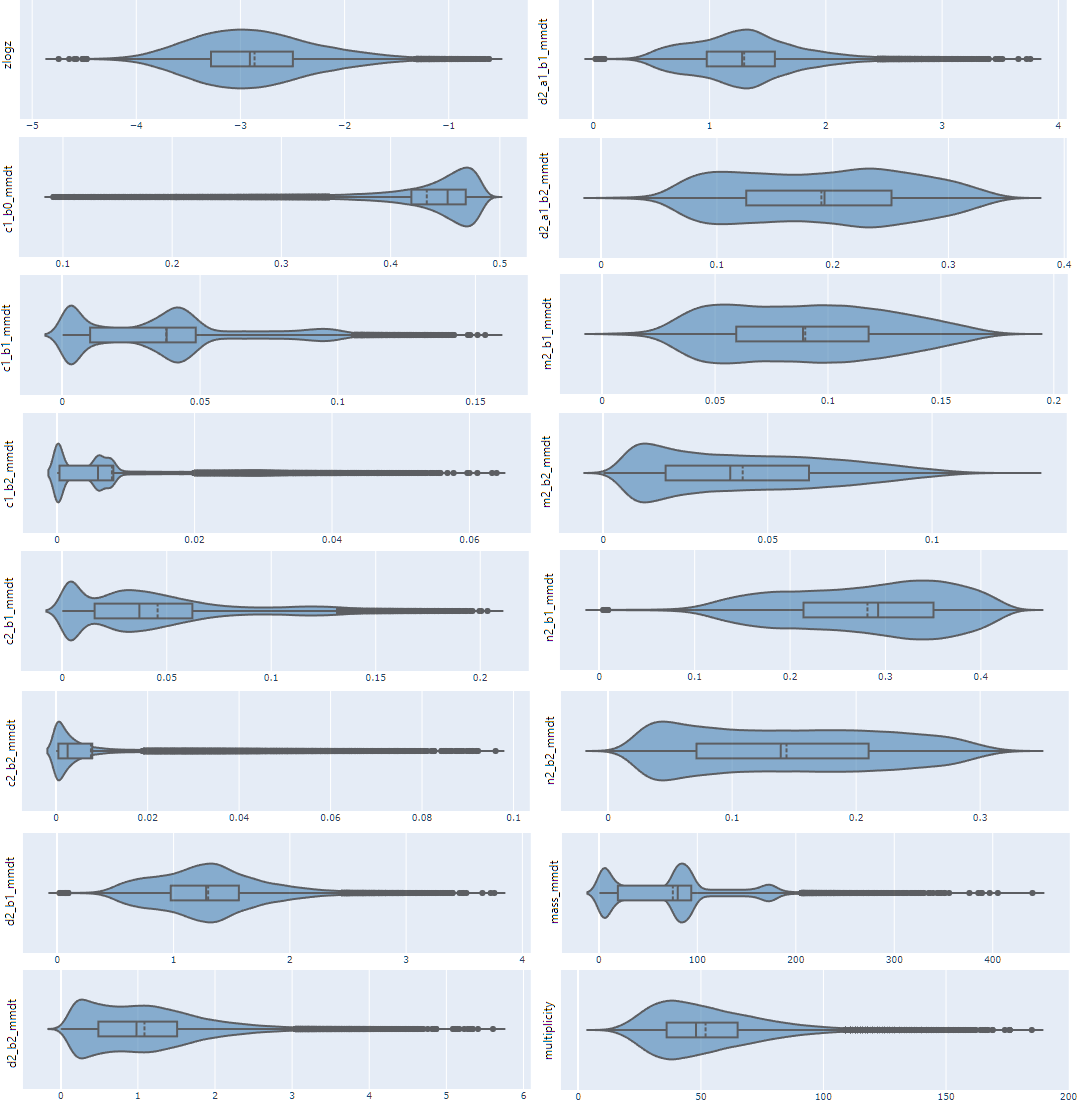
\includegraphics[trim={0cm 0cm 0cm 0cm}, width=1.0\textwidth, center]{background/distributions.png}
  \caption{Representation of the distributions of feature values in the HLF dataset.}
  \label{fig:distributions-hlf}
\end{figure}


\chapter{HLF dataset features distribution}
\begin{figure}[hpt!]
  \centering
  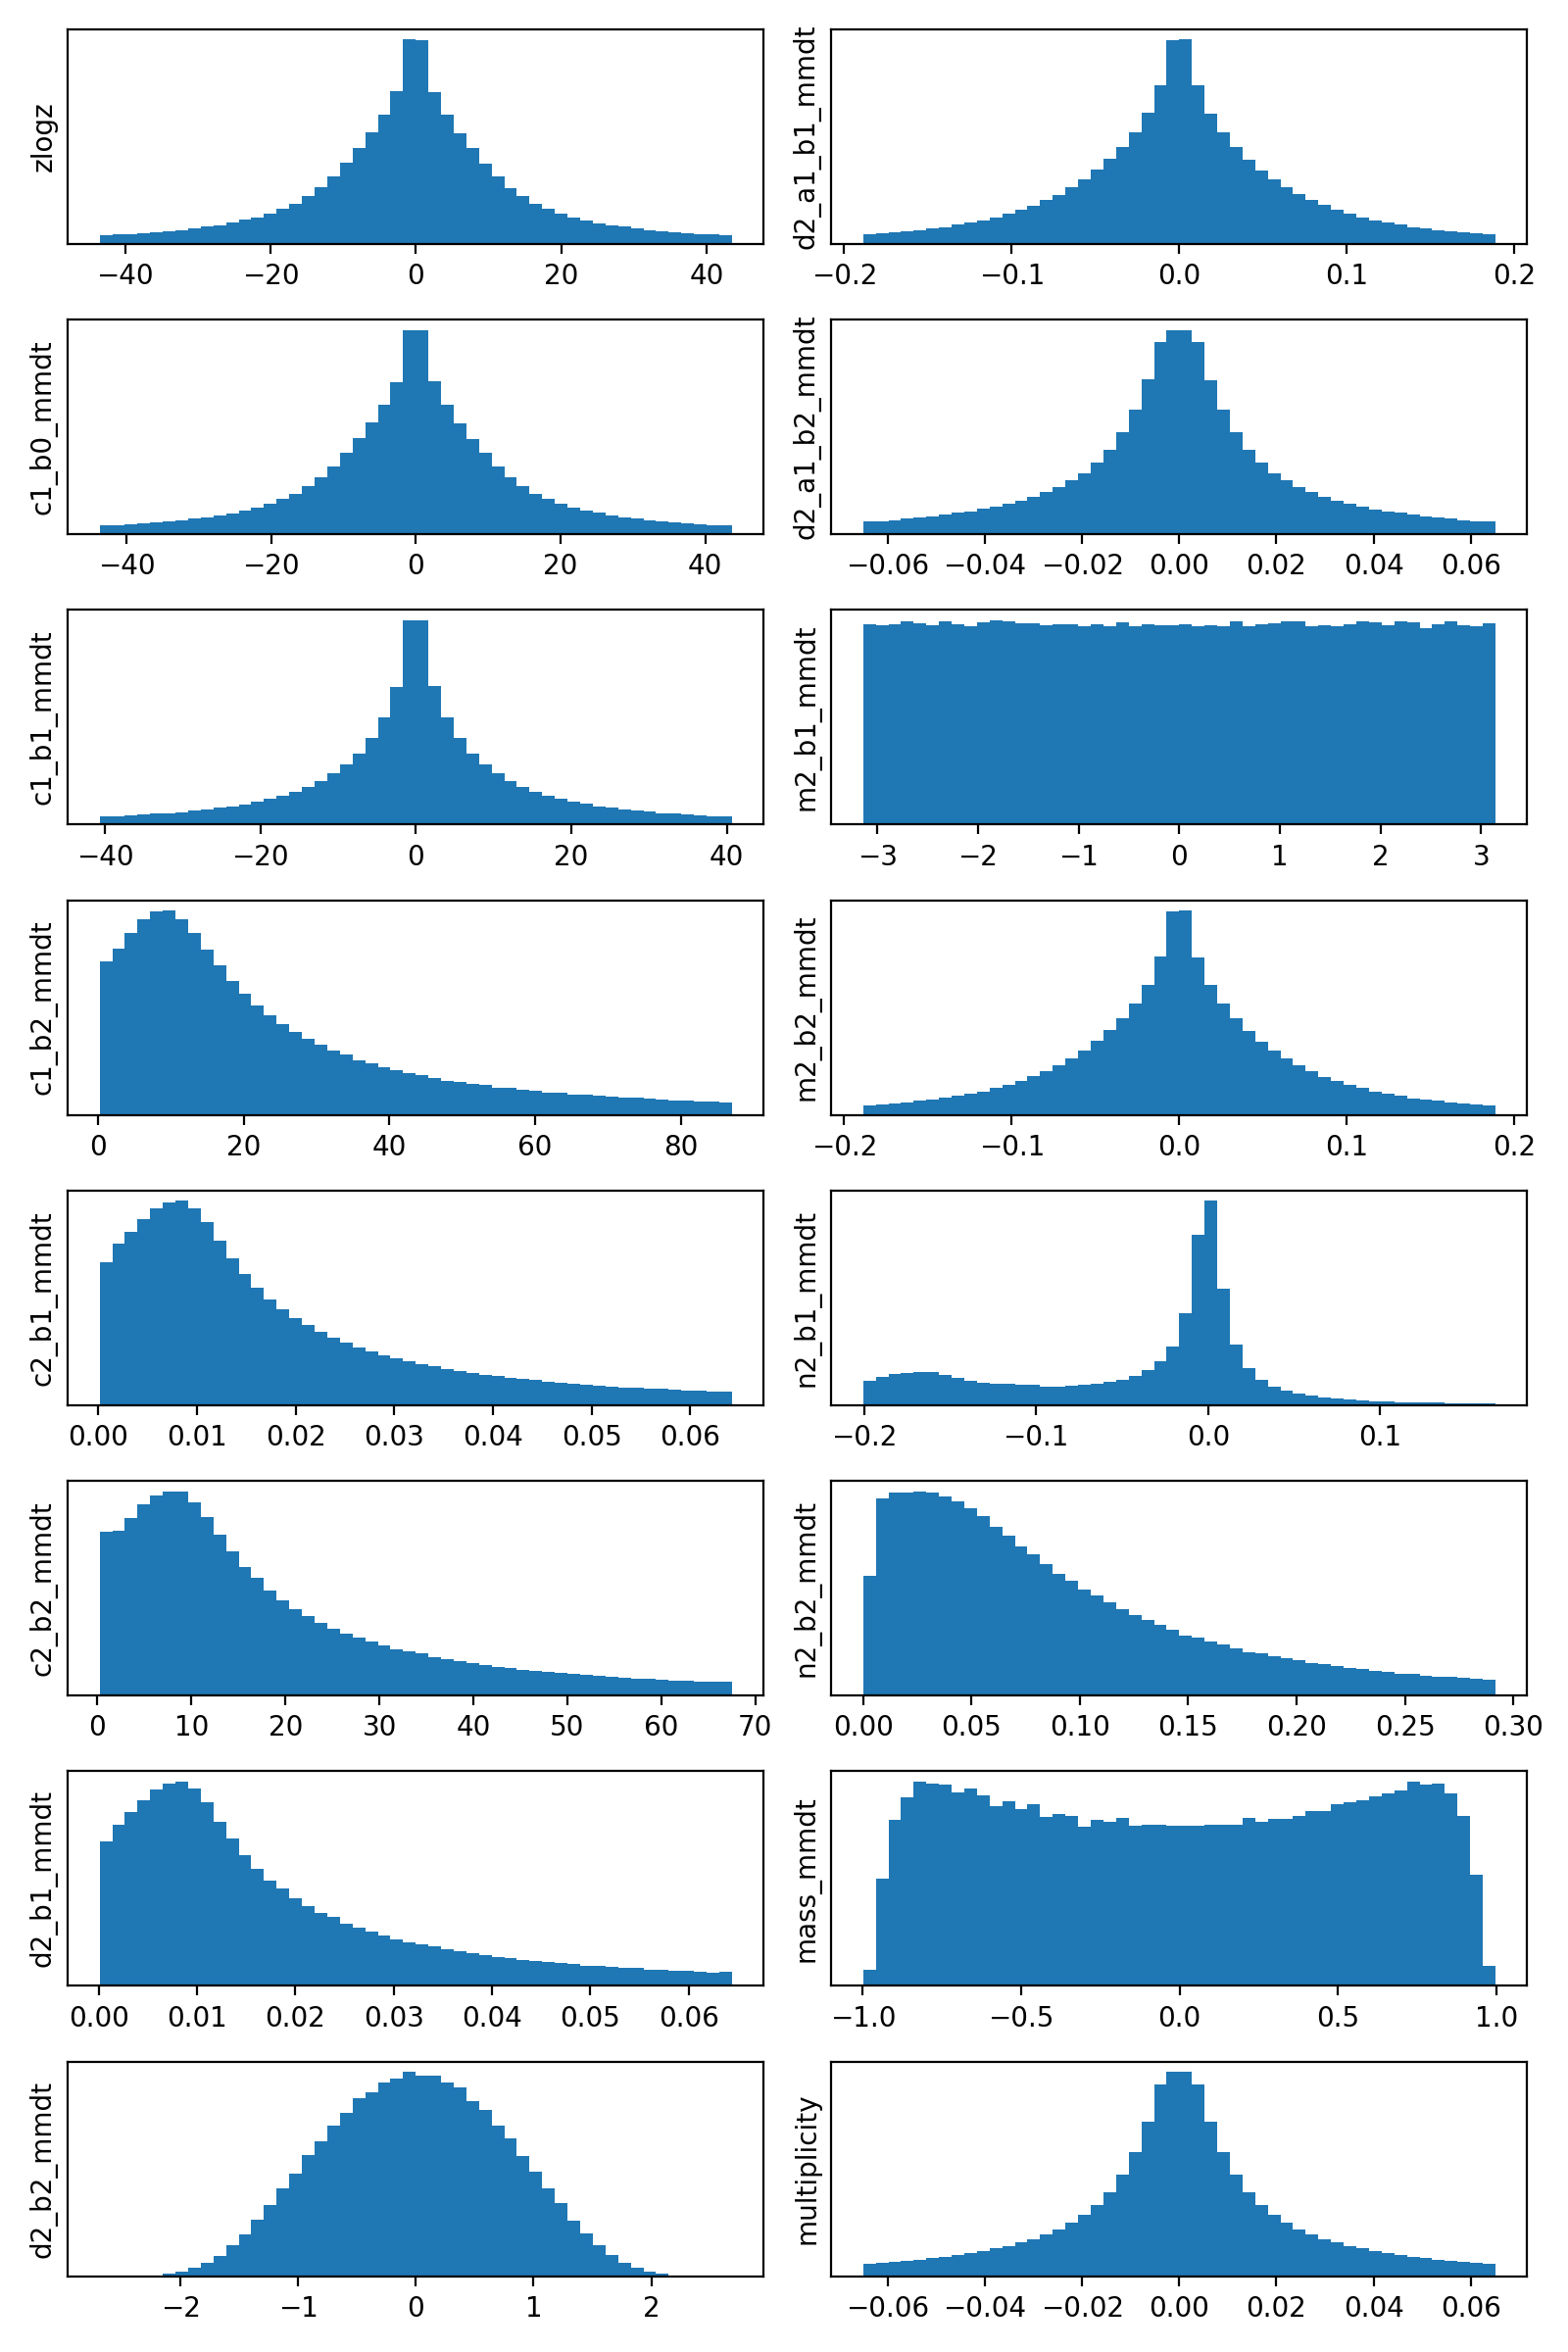
\includegraphics[trim={0cm 0cm 0cm 0cm}, width=0.7\textwidth, center]{../logs/constituent_distribution.png}
  \caption{Representation of the distributions of feature values in the constituent list dataset.}
  \label{fig:distributions-constituent}
\end{figure}

\end{appendices}